%%
%% ****** ljmsamp.tex 13.06.2018 ******
%%
\documentclass[
11pt,%
tightenlines,%
twoside,%
onecolumn,%
nofloats,%
nobibnotes,%
nofootinbib,%
superscriptaddress,%
noshowpacs,%
centertags]%
{revtex4}
\usepackage{ljm}

\begin{document}

\titlerunning{Surface remesh methods} % for running heads
\authorrunning{Rybakov} % for running heads
%\authorrunning{First-Author, Second-Author} % for running heads

\title{Estimation of surface remesh methods \\ in the ice accretion problem}
% Splitting into lines is performed by the command \\
% The title is written in accordance with the rules of capitalization.

\author{\firstname{A.~A.}~\surname{Rybakov}}
\email[E-mail: ]{rybakov_aan@nrcki.ru,rybakov@jscc.ru,rybakov.aax@gmail.com}
\affiliation{National Research Centre \textquotedblleft Kurchatov Institute\textquotedblright, 123182, Moscow, Academician Kurchatov sq. 1, Russia.}

%\author{\firstname{B.}~\surname{Second-Author}}
%\email[E-mail: ]{Second.Author@email.com}
%\affiliation{Place of work and/or the address of the first and second authors}
%\affiliation{Place of work and/or the address of second authors}
%\noaffiliation % If the author does not specify a place of work.

\firstcollaboration{(Submitted by TODO)} % Add if you know submitter.
%\lastcollaboration{ }

%\received{June 13, 2018} % The date of receipt to the editor, i.e. December 06, 2017

\begin{abstract} % You shouldn't use formulas and citations in the abstract.
The article considers the problem of rebuilding the surface computational mesh in the problem of ice accretion.
In this problem, the surface mesh should be rebuilt in accordance with the volume of ice accumulated in each mesh cell.
The main factor in choosing a mesh rebuilding method is the accuracy of the method, characterized by the magnitude of the deviation of the volume swept by the cell from the target value.
Another determining factor is the ability of the rebuilding method to smooth out mesh defects -- sharp peaks and caverns.
Without this, the computational mesh can accumulate defects, which sooner or later leads to the impossibility of continuing the calculations.
The paper considers theoretical estimates of three methods of rebuilding the surface mesh -- the rectangles method, the trapeziums method and the neighborhoods method - from the point of view of the accuracy of rebuilding and the ability to smooth out defects.
The results of the analysis showed that the rectangles and trapeziums methods cannot smooth out the defects of the computational mesh during rebuilding, which means that their use in the problem of ice formation is unsafe.
The neighborhoods method has an acceptable rebuilding accuracy and can smooth out the defects of the computational mesh. All results were obtained in a two-dimensional case, but the conclusions can be transferred to similar methods of rebuilding the surface mesh in a three-dimensional case.\end{abstract}

\subclass{68U05} % Enter 2010 Mathematics Subject Classification.

\keywords{rebuilding surface mesh, rectangles method, trapeziums method, neighborhoods method, rebuilding accuracy, smoothing sharp peaks and caverns} % Include keywords separeted by comma.

\maketitle

% Text of article starts here.

%--------------------------------------------------------------------------------------------------------------------------------

\section{Introduction}

Numerical modeling of the icing process of the surface is a complex multiphysical problem, including modeling of gas dynamics, heat exchange, liquid flow, droplet dynamics in the air flow, and others.
The study of ice formation processes is of great practical importance.
In particular, the nature and intensity of ice formation on the surface of an aircraft critically affects its flight characteristics, which is directly related to flight safety \cite{Raj}.

Today, the leader among foreign software for modeling the ice formation process is the ANSYS software package (including the FENSAP-ICE, DROP3D, ICE3D modules) \cite{Martini}.
In Russia, mathematical algorithms and software in this area are also being actively developed.
It is possible to note the research on the development of the iceFoam module as part of the open OpenFOAM package \cite{Koshelev}.
Among commercial products, the IceVision package as part of the FlowVision software package \cite{Sorokin} has been actively developing in recent years, as well as a solution as part of the LOGOS engineering analysis package \cite{Galanov}.

Modeling of the ice cover process is usually performed on a surface computational mesh and consists of two main parts.
The first part is the calculation of the ice growth rate in individual mesh cells (this can be the calculation of the mass of ice accumulated in each mesh cell per unit time, or the rate of ice cover formation at mesh nodes, or other similar characteristics).
To calculate the ice growth rate in mesh elements, there are many ice formation models that take into account different ice states, water film dynamics, heat flows, and other factors \cite{Bartkus,Zhang,Pena}.
Ice formation models are not considered in this paper.
The second important component of ice growth modeling is the determination of changes in the surface after the ice layer has grown on it.
This article analyzes methods for rebuilding a surface mesh in a two-dimensional formulation, for which three-dimensional analogs exist.

Let us consider the geometric problem of rebuilding a surface in two-dimensional space in general.
Let a surface mesh be given in the form of a polyline without self-intersections, each cell of which is represented by a segment of length $l_i$ ($0 \le i < n$).
For the $i$-th cell, the incident nodes are nodes with numbers $i$ and $i + 1$.
If nodes with numbers $0$ and $n$ coincide, then the mesh is closed.
The direction of the normal of each cell is known, as well as the direction of motion of each node, which coincides with the direction of the sum of unit normals drawn to the incident cells.
For the two-dimensional case, this direction lies on the bisector of the angle formed by two incident cells.
The angle between two adjacent cells with numbers $i - 1$ and $i$ will be denoted by $2 \phi_i$.
Let it be known that over a certain small period of time the $i$-th cell shifts in the direction of its normal by some value $H_i$, thus sweeping out an area $T_i = l_i H_i$, we will call this area the target area.
However, if we simply shift each cell in the direction of its normal, the mesh will lose its integrity, so we can only move the nodes.
It is required to find such values of local shifts of the mesh nodes $h_i$ ($0 \le i \le n$) that the swept area $S_i$ between the original surface and the new surface for each mesh cell differs as little as possible from the value of the target area $T_i$.
To estimate the deviation of the actual swept area from the target area, we will use the notations $\Delta_i = S_i - T_i$, $\delta_i = \frac{\Delta_i}{T_i}$.

When applied to the ice formation problem, the value $H_i$ corresponds to the thickness of the ice layer formed in the $i$-th cell \cite{Beaugendre}.
The new rebuilt surface mesh corresponds to the surface of the ice cover, and the total swept area during surface movement corresponds to the volume of ice accumulated on the surface \cite{Tong}.
The problem of finding the values of shifts of mesh nodes $h_i$ for fixed directions of displacement can be solved by the gradient descent method \cite{Rybakov}.
However, the gradient descent method turns out to be too demanding on computational resources as the mesh size increases.
In addition, the quality of the solution is often unsatisfactory when hitting local minima.
Therefore, approximate methods based on representing the target area in the form of primitive geometric figures can be used to solve the problem.

%--------------------------------------------------------------------------------------------------------------------------------

\section{Approximate methods of surface remeshing}

Let us consider approximate methods for rebuilding the computational mesh, based on representing the target area in the form of primitive geometric figures.

\begin{figure}[ht]
\setcaptionmargin{5mm}
%\onelinecaptionsfalse % if the caption is multiline
\onelinecaptionstrue  % if the caption is one-line
\begin{tabular}{ll}
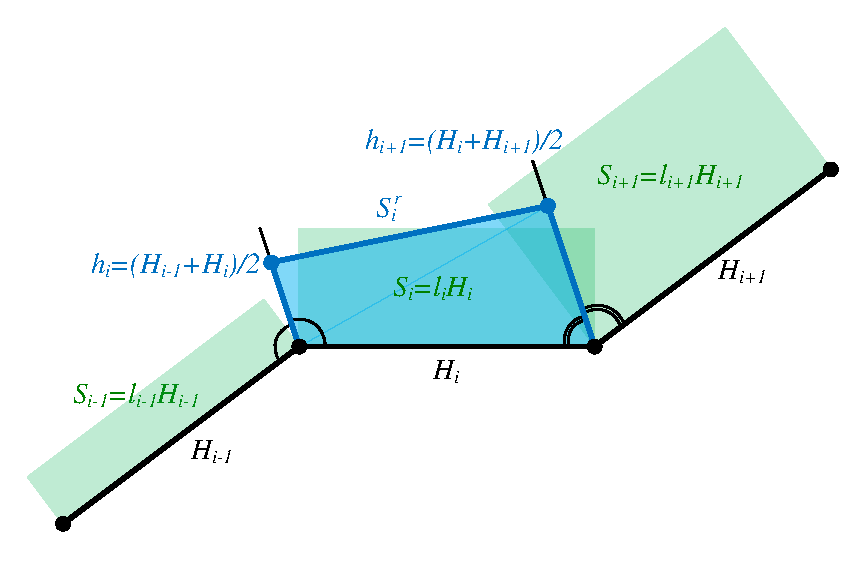
\includegraphics[width=0.45\textwidth]{pics/remesh_rectangles.pdf}
&
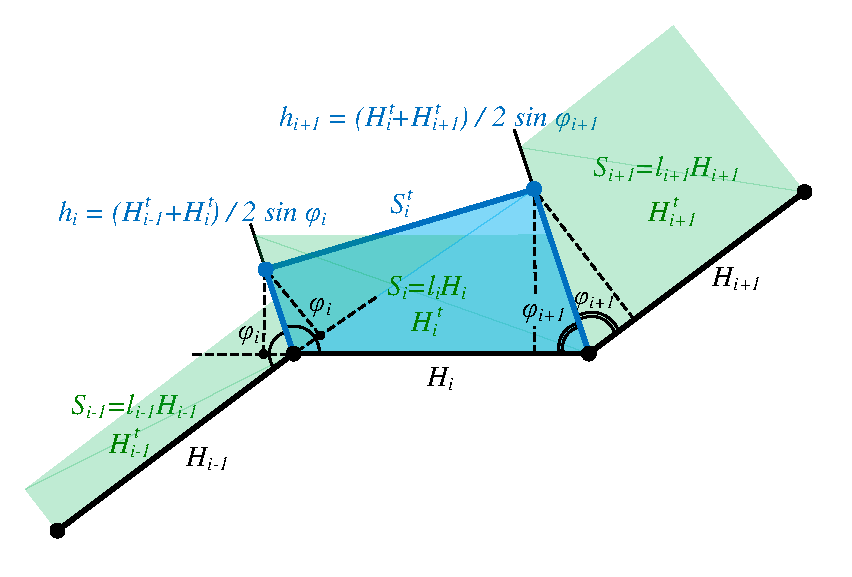
\includegraphics[width=0.45\textwidth]{pics/remesh_trapeziums.pdf}
\end{tabular}
\captionstyle{normal}\caption{Reconstruction of the surface using rectangles (left) and trapeziums (right).}
\label{fig:text_1_remesh_2d_rectangles_and_trapeziums}
\end{figure}

As the first method of remeshing the surface, we consider an approximation in which the target area for the $i$-th cell is represented by a rectangle with sides $l_i$ and $H_i$.
As the value of the node displacement, we take the arithmetic mean of two heights of the incident cells $h_i = \frac{H_{i - 1} + H_i}{2}$ (see Fig.~\ref{fig:text_1_remesh_2d_rectangles_and_trapeziums} on the left).
We will call this method of remeshing the rectangles method.
The area swept by the $i$-th cell using the rectangle method will be denoted by $S_i^r$, we also denote $\Delta_i^r = S_i^r - T_i$, $\delta_i^r = \frac{\Delta_i^r}{T_i}$.

As the second method of rebuilding the surface, we will consider the trapeziums method.
In the trapeziums method, the target area of the $i$-th cell is represented by a trapezium with area $T_i = l_i H_i$.
The lateral sides of this trapezium lie in the directions of motion of two nodes incident to the cell in question.
The height of the trapezium $H_i^t$ is found by solving a quadratic equation.
After constructing the trapeziums for all cells of the mesh, each node has two new potential positions for shifting (formed by the cell on the left and the cell on the right).
Their average value is selected as the final new position (Fig.~\ref{fig:text_1_remesh_2d_rectangles_and_trapeziums} on the right).
Thus, the magnitude of the node shift is determined as $h_i = \frac{H_{i - 1}^t + H_i^t}{2 \sin \phi_i}$.
The area swept by the $i$-th cell when using the trapeziums method will be denoted by $S_i^t$, and we will also denote $\Delta_i^t = S_i^t - T_i$, $\delta_i^t = \frac{\Delta_i^t}{T_i}$.
As a third method of mesh rebuilding, the neighborhoods method is considered, the description of which in a three-dimensional formulation can be found in \cite{Meshcheryakov}.
In this method, the mesh movement front is considered to determine new node positions (Fig.~\ref{fig:text_1_remesh_2d_okrestnost}).

\begin{figure}[ht]
\setcaptionmargin{5mm}
%\onelinecaptionsfalse % if the caption is multiline
\onelinecaptionstrue  % if the caption is one-line
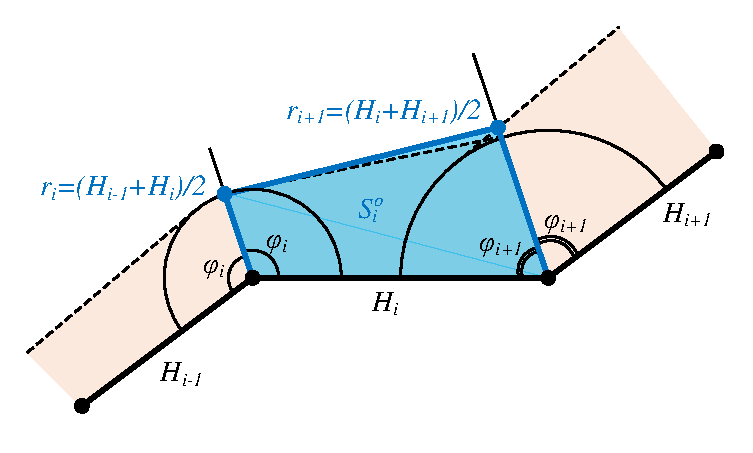
\includegraphics[width=0.6\textwidth]{pics/remesh_okrestnost.pdf}
\captionstyle{normal}\caption{Surface remeshing using the neighborhoods method.}
\label{fig:text_1_remesh_2d_okrestnost}
\end{figure}

In this case, the motion front of the node with the number $i$ is a sphere with the center at this node and the radius $r_i = \frac{H_{i - 1} + H_i}{2}$.
The motion front of a mesh cell is the convex hull of the motion fronts of two nodes incident to it.
Then the motion front of the mesh is the union of the motion fronts of all its cells.
As the new position of the node, we will take the intersection of the direction of displacement of the node and the boundary of the motion front of the mesh.
When using the neighborhoods method, we will denote the area swept by the $i$-th cell by $S_i^o$, and also denote $\Delta_i^o = S_i^o - T_i$, $\delta_i^o = \frac{\Delta_i^o}{T_i}$.

%--------------------------------------------------------------------------------------------------------------------------------

\section{Theoretical estimates of the accuracy of mesh rebuilding methods}

Let us present a theoretical estimate of the accuracy of approximate methods of remeshing.
The estimate will be performed for a model computational mesh that satisfies the following requirements.
All mesh cells are identical and have length $l$, the surface is convex.
For any cell $AB$ and its neighbors $A_2A$ and $BB_2$, the angles $\angle (\overline{BA}, \overline{AA_2})$ and $\angle (\overline{AB}, \overline{BB_2})$ are constant and equal to $\alpha$ (see Fig.~\ref{fig:text_1_remesh_2d_theoretical} on the left).
Let the displacements of cells $A_2A$, $AB$ and $BB_2$ be equal to $H_{i - 1}$, $H_i$ and $H_{i + 1}$, respectively.
\begin{figure}[ht]
\setcaptionmargin{5mm}
\onelinecaptionsfalse % if the caption is multiline
%\onelinecaptionstrue  % if the caption is one-line
\begin{tabular}{ll}
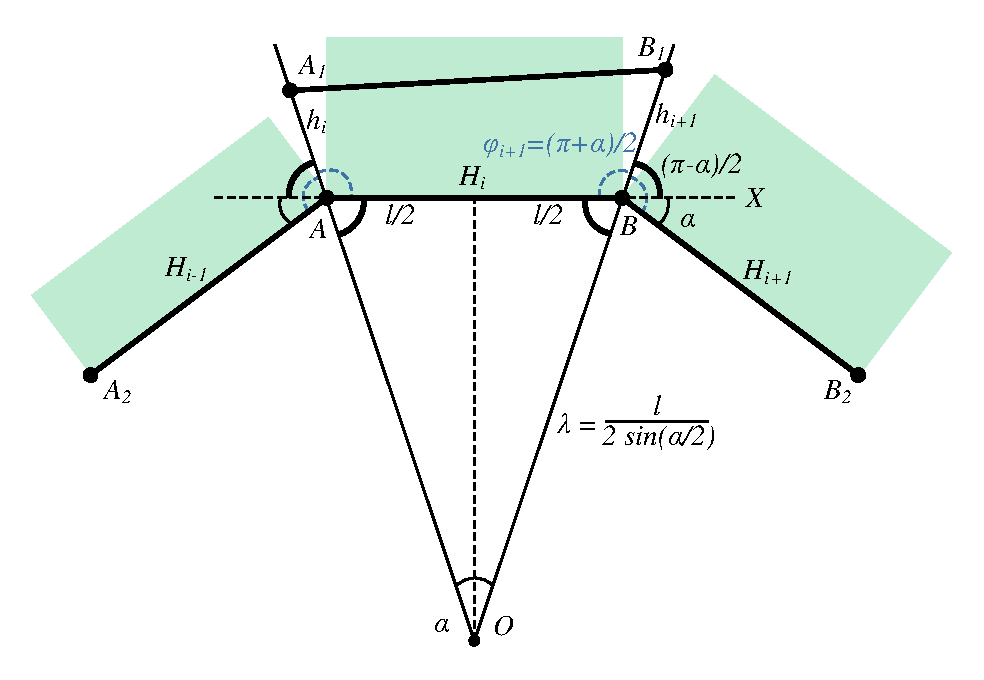
\includegraphics[width=0.45\textwidth]{pics/theoretical.pdf}
&
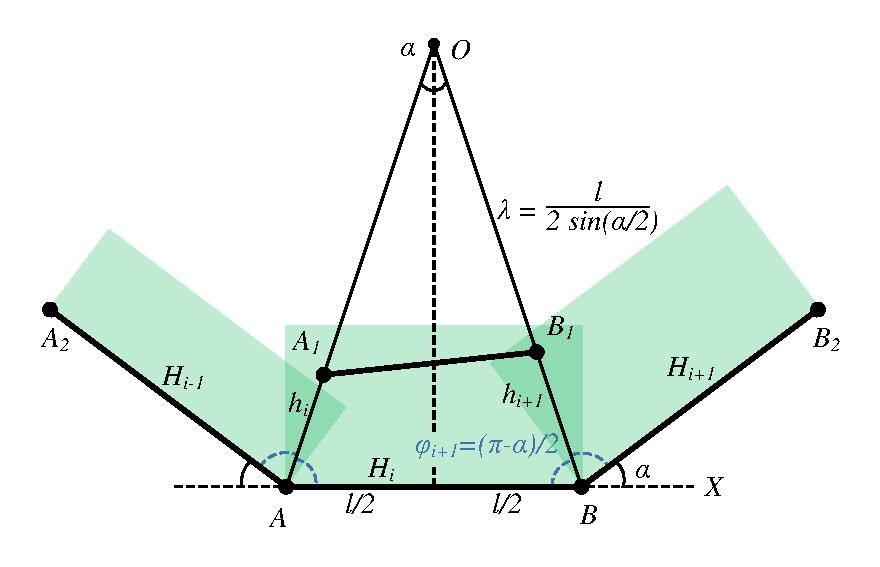
\includegraphics[width=0.45\textwidth]{pics/theoretical_concave.pdf}
\end{tabular}
\captionstyle{normal}\caption{Theoretical evaluation of approximate methods for rebuilding convex (left) and concave (right) meshes.}
\label{fig:text_1_remesh_2d_theoretical}
\end{figure}

To calculate the values $\Delta$, $\delta$ it is necessary to calculate the area $S_i = S_{AA_1B_1B}$.
When using different remeshing methods this area will differ.

\begin{lemma}\label{lem:text_1_remesh2_vypukl_lemma}
For a cell $AB$ of a convex mesh with equal angles $\angle (\overline{BA}, \overline{AA_2}) = \angle (\overline{AB}, \overline{BB_2}) = \alpha$ (see Fig.~\ref{fig:text_1_remesh_2d_theoretical})
\begin{equation}\label{eqn:text_1_remesh2_saa2b2b_gen}
S_i(h_i, h_{i + 1}) = \frac{1}{2} \sin \alpha \left( \lambda(h_i + h_{i+1}) + h_ih_{i+1} \right)
\end{equation}
where $\lambda = \frac{l}{2 \sin \frac{\alpha}{2}}$, $l = AB$, $h_i = AA_1$, $h_{i + 1} = BB_1$.
\end{lemma}

Since the mesh under consideration is convex, the rays $A_1A$ and $B_1B$ intersect at some point $O$.
In this case, the triangle $AOB$ is isosceles, $\angle BAO = \angle ABO = \angle B_1BX = \angle B_1BB_2 - \alpha = \frac{\pi - \alpha}{2}$, $\phi_i = \phi_{i + 1} = \frac{\pi + \alpha}{2}$, $\angle AOB = \alpha$, whence $OA = OB = \lambda = \frac{l}{2 \sin \frac{\alpha}{2}}$.
Next we express the area $S_i = S_{A_1OB_1} - S_{AOB}$, which after transformation gives the required ratio \eqref{eqn:text_1_remesh2_saa2b2b_gen}.$\blacksquare$\\

Next, we will consider a linear change in the magnitude of the mesh cell displacement, that is, $H_i = H$, $H_{i - 1} = H - \Delta H$, $H_{i + 1} = H + \Delta H$.

For remeshing by the rectangles method we have $h_i = H - \frac{1}{2} \Delta H$, $h_{i + 1} = H + \frac{1}{2} \Delta H$, whence
\begin{equation}\label{eqn:text_1_remesh2_s_rect}
	S_i^r = \cos \frac{\alpha}{2} \left( lH + \left( H^2 - \frac{1}{4} \Delta H^2 \right) \sin \frac{\alpha}{2} \right)
\end{equation}

Now let's move on to calculating $S_i^t$ for the trapeziums method.
In the trapeziums method, we must represent the target areas in cells $A_2A$, $AB$, $BB_2$ using isosceles trapeziums for which one of the bases is known (the same for all cells and equal to $l$), the angle at this base (the same for all cells and equal to $\phi = \frac{\pi + \alpha}{2}$, and the areas of these trapeziums, equal to $T_{i - 1} = l(H - \Delta H)$, $T_i = lH$ and $T_{i + 1} = l(H + \Delta H)$, respectively.
Based on this data, it is necessary to calculate the heights of the trapeziums, which can be done by solving a quadratic equation.
Let's denote the heights of these trapeziums:
\begin{equation}
	\begin{aligned}\label{eqn:text_1_remesh_2_Ht_vypukl}
		& H_{i - 1}^t = H^t\left(l(H - \Delta H), l, \frac{\pi + \alpha}{2}\right) \\ 
		& H_i^t = H^t\left(lH, l, \frac{\pi + \alpha}{2}\right) \\
		& H_{i + 1}^t = H^t\left(l(H + \Delta H), l, \frac{\pi + \alpha}{2}\right)
	\end{aligned}
\end{equation}

Then $h_i = \frac{H_{i - 1}^t + H_i^t}{2 \sin \phi_i} = \frac{H_{i - 1}^t + H_i^t}{2 \cos \frac{\alpha}{2}}$, $h_{i+1} = \frac{H_i^t + H_{i+1}^t}{2 \sin \phi_{i + 1}} = \frac{H_i^t + H_{i+1}^t}{2 \cos \frac{\alpha}{2}}$ and the expression \eqref{eqn:text_1_remesh2_saa2b2b_gen} for $S_i^t$ takes the following form:
\begin{equation}\label{eqn:text_1_remesh2_trap}
	S_i^t = \frac{1}{4} \left( (H_{i - 1}^t + 2 H_i^t + H_{i + 1}^t)l + (H_{i - 1}^t + H_i^t) (H_i^t + H_{i+1}^t) \tg \frac{\alpha}{2} \right)
\end{equation}

To obtain a theoretical estimate of the accuracy for the neighborhoods method in the case of a convex mesh, consider the following auxiliary statement (see Fig.~\ref{fig:text_1_remesh_2d_accuracy_okrestnost} on the left).

\begin{figure}[ht]
\setcaptionmargin{5mm}
\onelinecaptionsfalse % if the caption is multiline
%\onelinecaptionstrue  % if the caption is one-line
\begin{tabular}{ll}
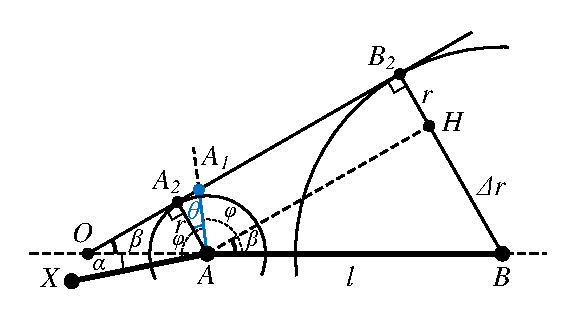
\includegraphics[width=0.45\textwidth]{pics/accuracy_okrestnost.pdf}
&
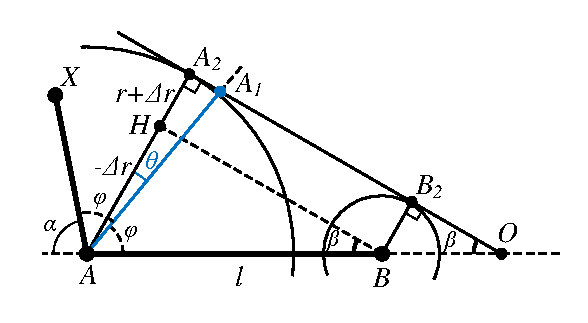
\includegraphics[width=0.45\textwidth]{pics/accuracy_okrestnost2.pdf}
\end{tabular}
\captionstyle{normal}\caption{Calculation of node displacement in the neighborhoods method for a convex (left) and concave (right) mesh.}
\label{fig:text_1_remesh_2d_accuracy_okrestnost}
\end{figure}

\begin{lemma}\label{lem:text_1_remesh_2d_accuracy_okrestnost}
Let $AB = l$, below the line $AB$ there is a point $X$ such that $\angle (\overline{AX}, \overline{BA}) = \alpha$.
Let two circles be constructed with centers at points $A$ and $B$ and with radii $r$ and $r + \Delta r$, respectively.
For the constructed circles, a convex hull is constructed consisting of arcs of these circles, as well as segments of common tangents (the points of tangency of the common tangent of the constructed circles, lying above the line $AB$, are denoted by $A_2$ and $B_2$, respectively).
Let this convex hull -- either on the circle with center at point $A$ or on the segment $A_2B_2$ -- contain a point $A_1$ such that $\angle XAA_1 = \angle BAA_1 = \phi$, $AA_1 = h$, then
\begin{equation}
	\begin{cases}\label{eqn:text_1_remesh_2d_okr_h}
		h = r, \  \sin \frac{\alpha}{2} > \frac{\Delta r}{l}, \\
		h(\alpha, l, r, \Delta r) = \frac{r}{\cos \left( \arcsin \frac{\Delta r}{l} - \frac{\alpha}{2} \right)}, \  \sin \frac{\alpha}{2} \le \frac{\Delta r}{l}
	\end{cases}
\end{equation}
\end{lemma}

If point $A_1$ is not on segment $A_2B_2$, then $h = AA_1 = r$.

Consider the case when $A_1$ is on the segment $A_2B_2$, in which case $\Delta r > 0$.
Through point $A$ we draw a line parallel to $A_2B_2$ until it intersects $BB_2$ at point $H$.
Then $\angle B_2OB = \angle HAB = \beta = \arcsin \frac{\Delta r}{l}$.
Since $\angle A_1AB = \phi = \frac{\pi + \alpha}{2}$, then $\angle OAA_2 + \theta + \phi = \pi$, whence we obtain $\theta = \beta - \frac{\alpha}{2}$.

Thus, the condition for finding the point $A_1$ on the segment $A_2B_2$ is equivalent to $\theta \ge 0$.
That is, for $\theta < 0$, we obtain $h = r$, and for $\theta \ge 0$, the value of $h$ can be expressed from the right triangle $AA_1A_2$.
$\blacksquare$\\

Using the lemma~\ref{lem:text_1_remesh_2d_accuracy_okrestnost}, $S_i^o$ from \eqref{eqn:text_1_remesh2_saa2b2b_gen} can be expressed for the neighborhoods method by substituting there the expressions for $h_i$ and $h_{i + 1}$ from \eqref{eqn:text_1_remesh_2d_okr_h}:
\begin{equation}
	\begin{aligned}
	& h_i = h \left( \alpha, l, H - \frac{1}{2}\Delta H, \Delta H \right) \\
	& h_{i + 1} = h \left( \alpha, l, H + \frac{1}{2}\Delta H, \Delta H \right)
	\end{aligned}
\end{equation}

Now consider the case of a concave mesh, shown in Fig.~\ref{fig:text_1_remesh_2d_theoretical} on the right.

\begin{lemma}
For a cell $AB$ of a concave mesh with equal angles $\angle (\overline{BA}, \overline{AA_2}) = \angle (\overline{AB}, \overline{BB_2}) = \alpha$ (see Fig.~\ref{fig:text_1_remesh_2d_theoretical} on the right)
\begin{equation}\label{eqn:text_1_remesh2_saa2b2b_gen2}
S_i = \frac{1}{2} \sin \alpha \left( \lambda(h_i + h_{i+1}) - h_ih_{i+1} \right)
\end{equation}
where $\lambda = \frac{1}{2 \sin \frac{\alpha}{2}}$, $l = AB$, $h_i = AA_1$, $h_{i + 1} = BB_1$, and the formula \eqref{eqn:text_1_remesh2_saa2b2b_gen2} is applicable if at least one of the conditions $h_i \le \lambda$, $h_{i+1} \le \lambda$ is met.
\end{lemma}

The calculations are performed similarly to the lemma~\ref{lem:text_1_remesh2_vypukl_lemma}, with the only difference that $S_i = S_{AOB} - S_{A_1OB_1}$, from which we have the expression \eqref{eqn:text_1_remesh2_saa2b2b_gen2}.

Fulfillment of at least one of the conditions $h_i \le \lambda$, $h_{i+1} \le \lambda$ is necessary to prevent self-intersection of the mesh.
$\blacksquare$\\

For reconstruction by the rectangles method and the trapeziums method in the case of a concave mesh, we obtain formulas similar to \eqref{eqn:text_1_remesh2_s_rect}, \eqref{eqn:text_1_remesh_2_Ht_vypukl} and \eqref{eqn:text_1_remesh2_trap}:
\begin{equation}\label{eqn:text_1_remesh2_s_rect_vogn}
	S_i^r = \cos \frac{\alpha}{2} \left( lH - \left( H^2 - \frac{1}{4} \Delta H^2 \right) \sin \frac{\alpha}{2} \right) \\
\end{equation}
\begin{equation}\label{eqn:text_1_remesh_2_Ht_vogn}
	\begin{aligned}
	& H_{i - 1}^t = H^t\left(l(H - \Delta H), l, \frac{\pi - \alpha}{2}\right) \\ 
	& H_i^t = H^t\left(lH, l, \frac{\pi - \alpha}{2}\right) \\
	& H_{i + 1}^t = H^t\left(l(H + \Delta H), l, \frac{\pi - \alpha}{2}\right)
	\end{aligned}
\end{equation}
\begin{equation}\label{eqn:text_1_remesh2_trap_vogn}
	S_i^t = \frac{1}{4} \left( (H_{i - 1}^t + 2 H_i^t + H_{i + 1}^t)l - (H_{i - 1}^t + H_i^t) (H_i^t + H_{i+1}^t) \tg \frac{\alpha}{2} \right)
\end{equation}

Note that the formulas \eqref{eqn:text_1_remesh2_s_rect_vogn} -- \eqref{eqn:text_1_remesh2_trap_vogn} are identical to the formulas \eqref{eqn:text_1_remesh2_s_rect} -- \eqref{eqn:text_1_remesh2_trap} taking into account the sign of $\alpha$, therefore the formulas \eqref{eqn:text_1_remesh2_s_rect} -- \eqref{eqn:text_1_remesh2_trap} are applicable both for positive values of the angles $\alpha$ (the case of a convex mesh) and for negative values of $\alpha$ (the case of a concave mesh).

To obtain a theoretical estimate of the accuracy for the neighborhoods method in the case of a concave mesh, we consider the following auxiliary statement, similar to Lemma~\ref{lem:text_1_remesh_2d_accuracy_okrestnost} (see Fig.~\ref{fig:text_1_remesh_2d_accuracy_okrestnost} on the right).

\begin{lemma}\label{lem:text_1_remesh_2d_accuracy_okrestnost2}
Let $AB = l$, and let $X$ be located above the line $AB$ such that $\angle (\overline{AX}, \overline{BA}) = \alpha$.
Let two circles be constructed with centers at points $A$ and $B$ and with radii $r$ and $r + \Delta r$, respectively.
A convex hull is constructed for the constructed circles, consisting of arcs of these circles, as well as segments of common tangents (the points of tangency of the common tangent of the constructed circles, lying above the line $AB$, are denoted by $A_2$ and $B_2$, respectively).
Let this convex hull -- either on the circle with center at point $A$ or on the segment $A_2B_2$ -- contain a point $A_1$ such that $\angle XAA_1 = \angle BAA_1 = \phi$, $AA_1 = h$, then
\begin{equation}
	\begin{cases}\label{eqn:text_1_remesh_2d_okr_h2}
		h = r, \ \sin \frac{\alpha}{2} < \frac{-\Delta r}{l}, \\
		h(\alpha, l, r, \Delta r) = \frac{r}{\cos \left( \frac{\alpha}{2} - \arcsin \frac{-\Delta r}{l} \right)}, \ \sin \frac{\alpha}{2} \ge \frac{-\Delta r}{l}
	\end{cases}
\end{equation}
\end{lemma}

If point $A_1$ is not on segment $A_2B_2$, then $h = AA_1 = r$.

Let us consider the case when $A_1$ is on the segment $A_2B_2$, in which case $\Delta r < 0$.
Through point $B$ we draw a line parallel to $A_2B_2$ until it intersects $AA_2$ at point $H$.
Then $\angle A_2OA = \angle HBA = \beta = \arcsin \frac{-\Delta r}{l}$.
Since $\angle A_1AB = \phi = \frac{\pi - \alpha}{2}$, then $\angle A_2AA_1 = \theta = \angle A_2AO - \phi = \frac{\alpha}{2} - \beta$.

Thus, the condition for finding the point $A_1$ on the segment $A_2B_2$ is equivalent to $\theta \ge 0$.
That is, for $\theta < 0$, we obtain $h = r$, and for $\theta \ge 0$, the value of $h$ can be expressed from the right triangle $AA_1A_2$.
$\blacksquare$\\

Using the lemma~\ref{lem:text_1_remesh_2d_accuracy_okrestnost2}, for the neighborhoods method we can express $S_i^o$ from \eqref{eqn:text_1_remesh2_saa2b2b_gen2} by substituting there the expressions for $h_i$ and $h_{i + 1}$ from \eqref{eqn:text_1_remesh_2d_okr_h2}:
\begin{equation}
	\begin{aligned}
	& h_i = \max \left( h \left( \alpha, l, H - \frac{3}{2}\Delta H, \Delta H \right), h \left( \alpha, l, H - \frac{1}{2}\Delta H, \Delta H \right) \right) \\
	& h_{i + 1} = \max \left( h \left( \alpha, l, H - \frac{1}{2}\Delta H, \Delta H \right), h \left( \alpha, l, H + \frac{1}{2}\Delta H, \Delta H \right) \right)
	\end{aligned}
\end{equation}

Using the obtained relations for $S_i^r$, $S_i^t$, $S_i^o$, we can analyze the dependences of the quantities $\delta_i^r$, $\delta_i^t$, $\delta_i^o$ on $\alpha$ and $\frac{\Delta H}{l}$, while we will use the fixed quantity $H = \frac{l}{2}$ (see Fig.~\ref{fig:text_1_remesh_3d_main_chart}).

\begin{figure}[ht]
\setcaptionmargin{5mm}
%\onelinecaptionsfalse % if the caption is multiline
\onelinecaptionstrue  % if the caption is one-line
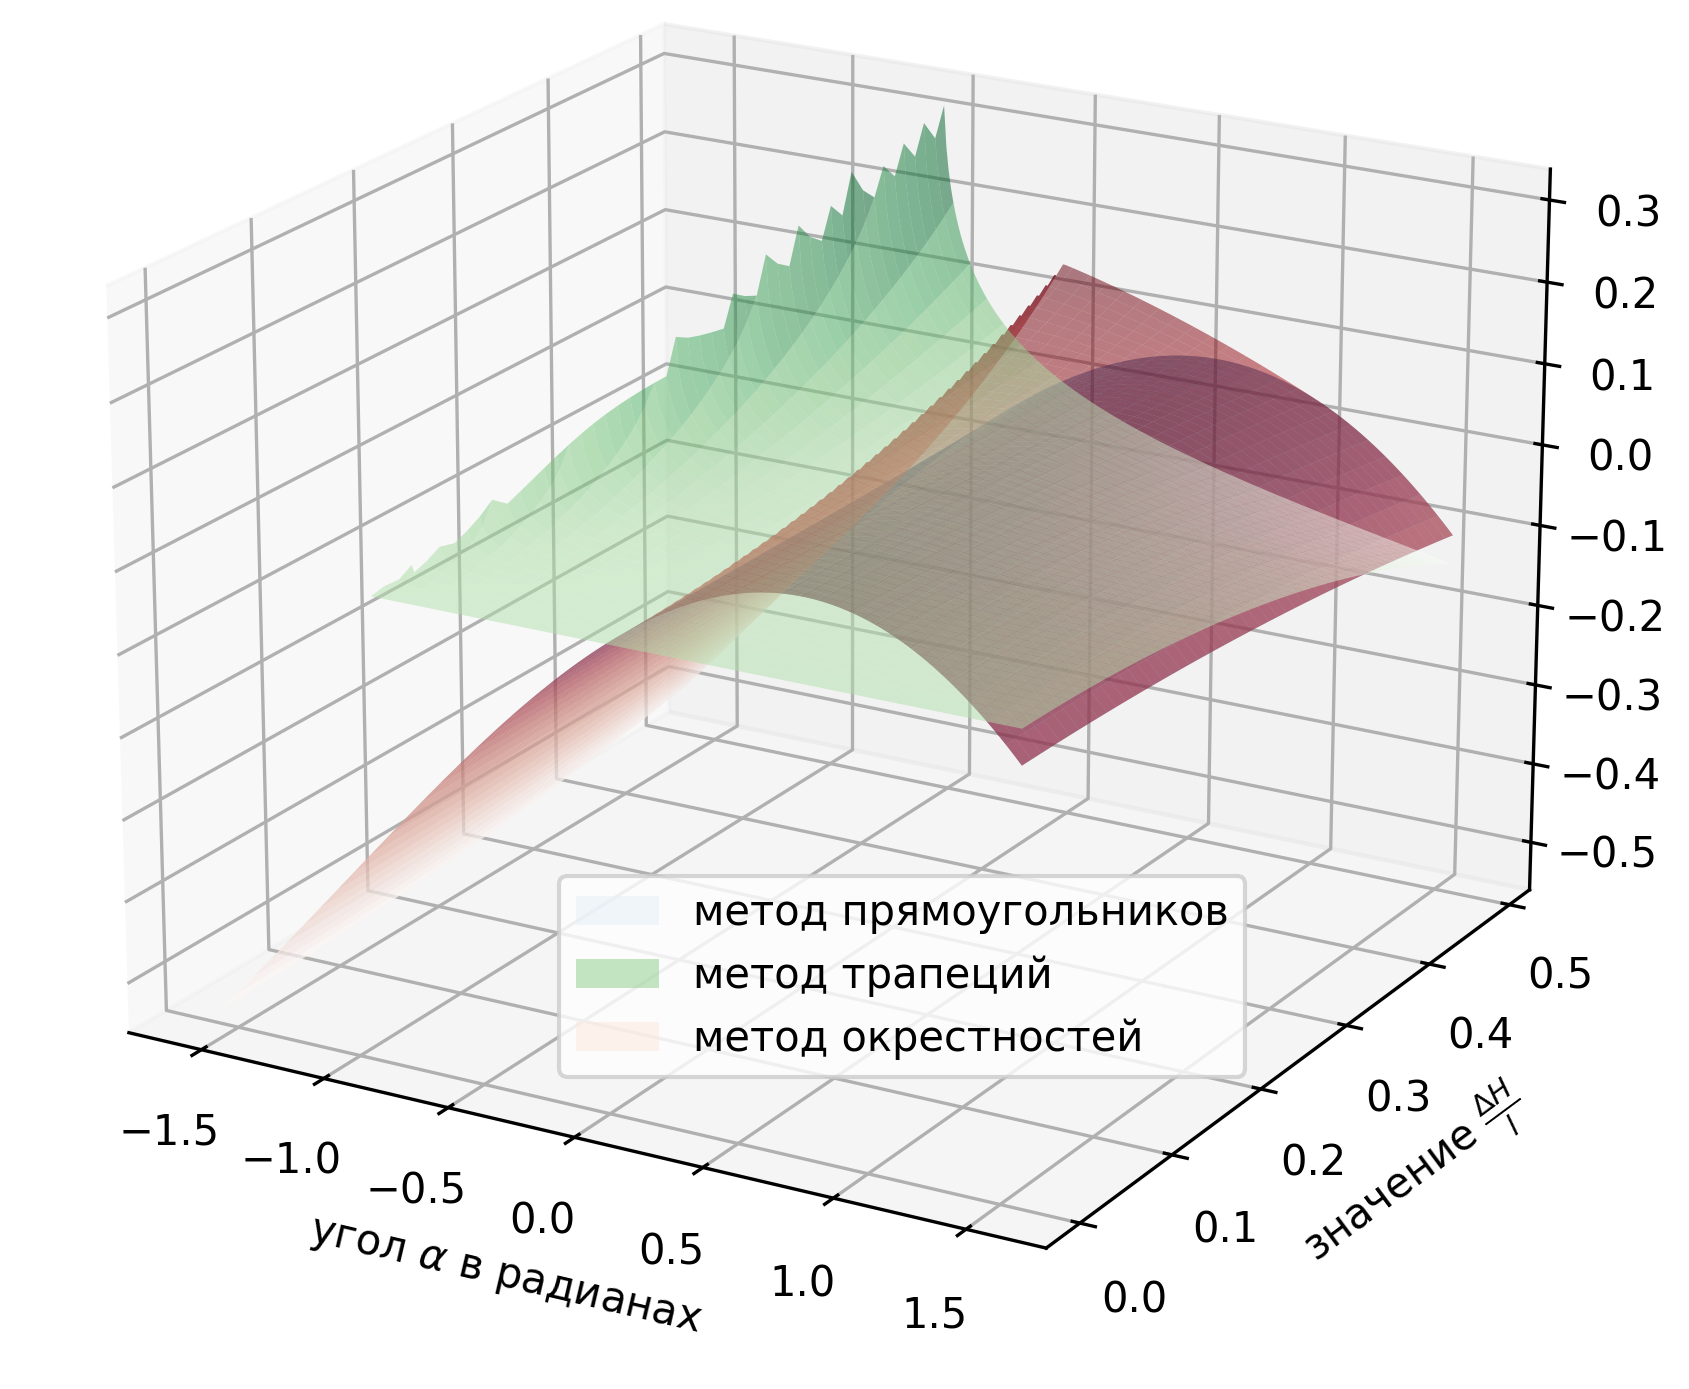
\includegraphics[width=0.8\textwidth]{pics/remesh_3d_chart.png}
\captionstyle{normal}\caption{Vizualization of $\delta_i^r(\alpha, \frac{\Delta H}{l})$, $\delta_i^t(\alpha, \frac{\Delta H}{l})$, $\delta_i^o(\alpha, \frac{\Delta H}{l})$ for a fixed value of $H = \frac{l}{2}$.}
\label{fig:text_1_remesh_3d_main_chart}
\end{figure}

From Fig.~\ref{fig:text_1_remesh_3d_main_chart} it can be noted that for $\Delta H = 0$ the trapeziums method is absolutely accurate by definition.
We also note that for $\Delta H = 0$ the deviations $\delta_i^r$ and $\delta_i^o$ are almost identical.

Let us additionally construct two graphs of the dependences of $\delta_i^r$, $\delta_i^t$, $\delta_i^o$ on $\frac{\Delta H}{l}$ for fixed values of $\alpha = 0.5$ (for a convex mesh) and $\alpha = -0.5$ (for a concave mesh) (see Fig.~\ref{fig:text_1_remesh_fix_alfa_chart}).
It is evident from the figure that the trapeziums method of rebuilding the surface for small values of $\frac{\Delta H}{l}$ is the most accurate, while the accuracy of the rectangle and neighborhoods methods is quite close.

\begin{figure}[ht]
\setcaptionmargin{5mm}
\onelinecaptionsfalse % if the caption is multiline
%\onelinecaptionstrue  % if the caption is one-line
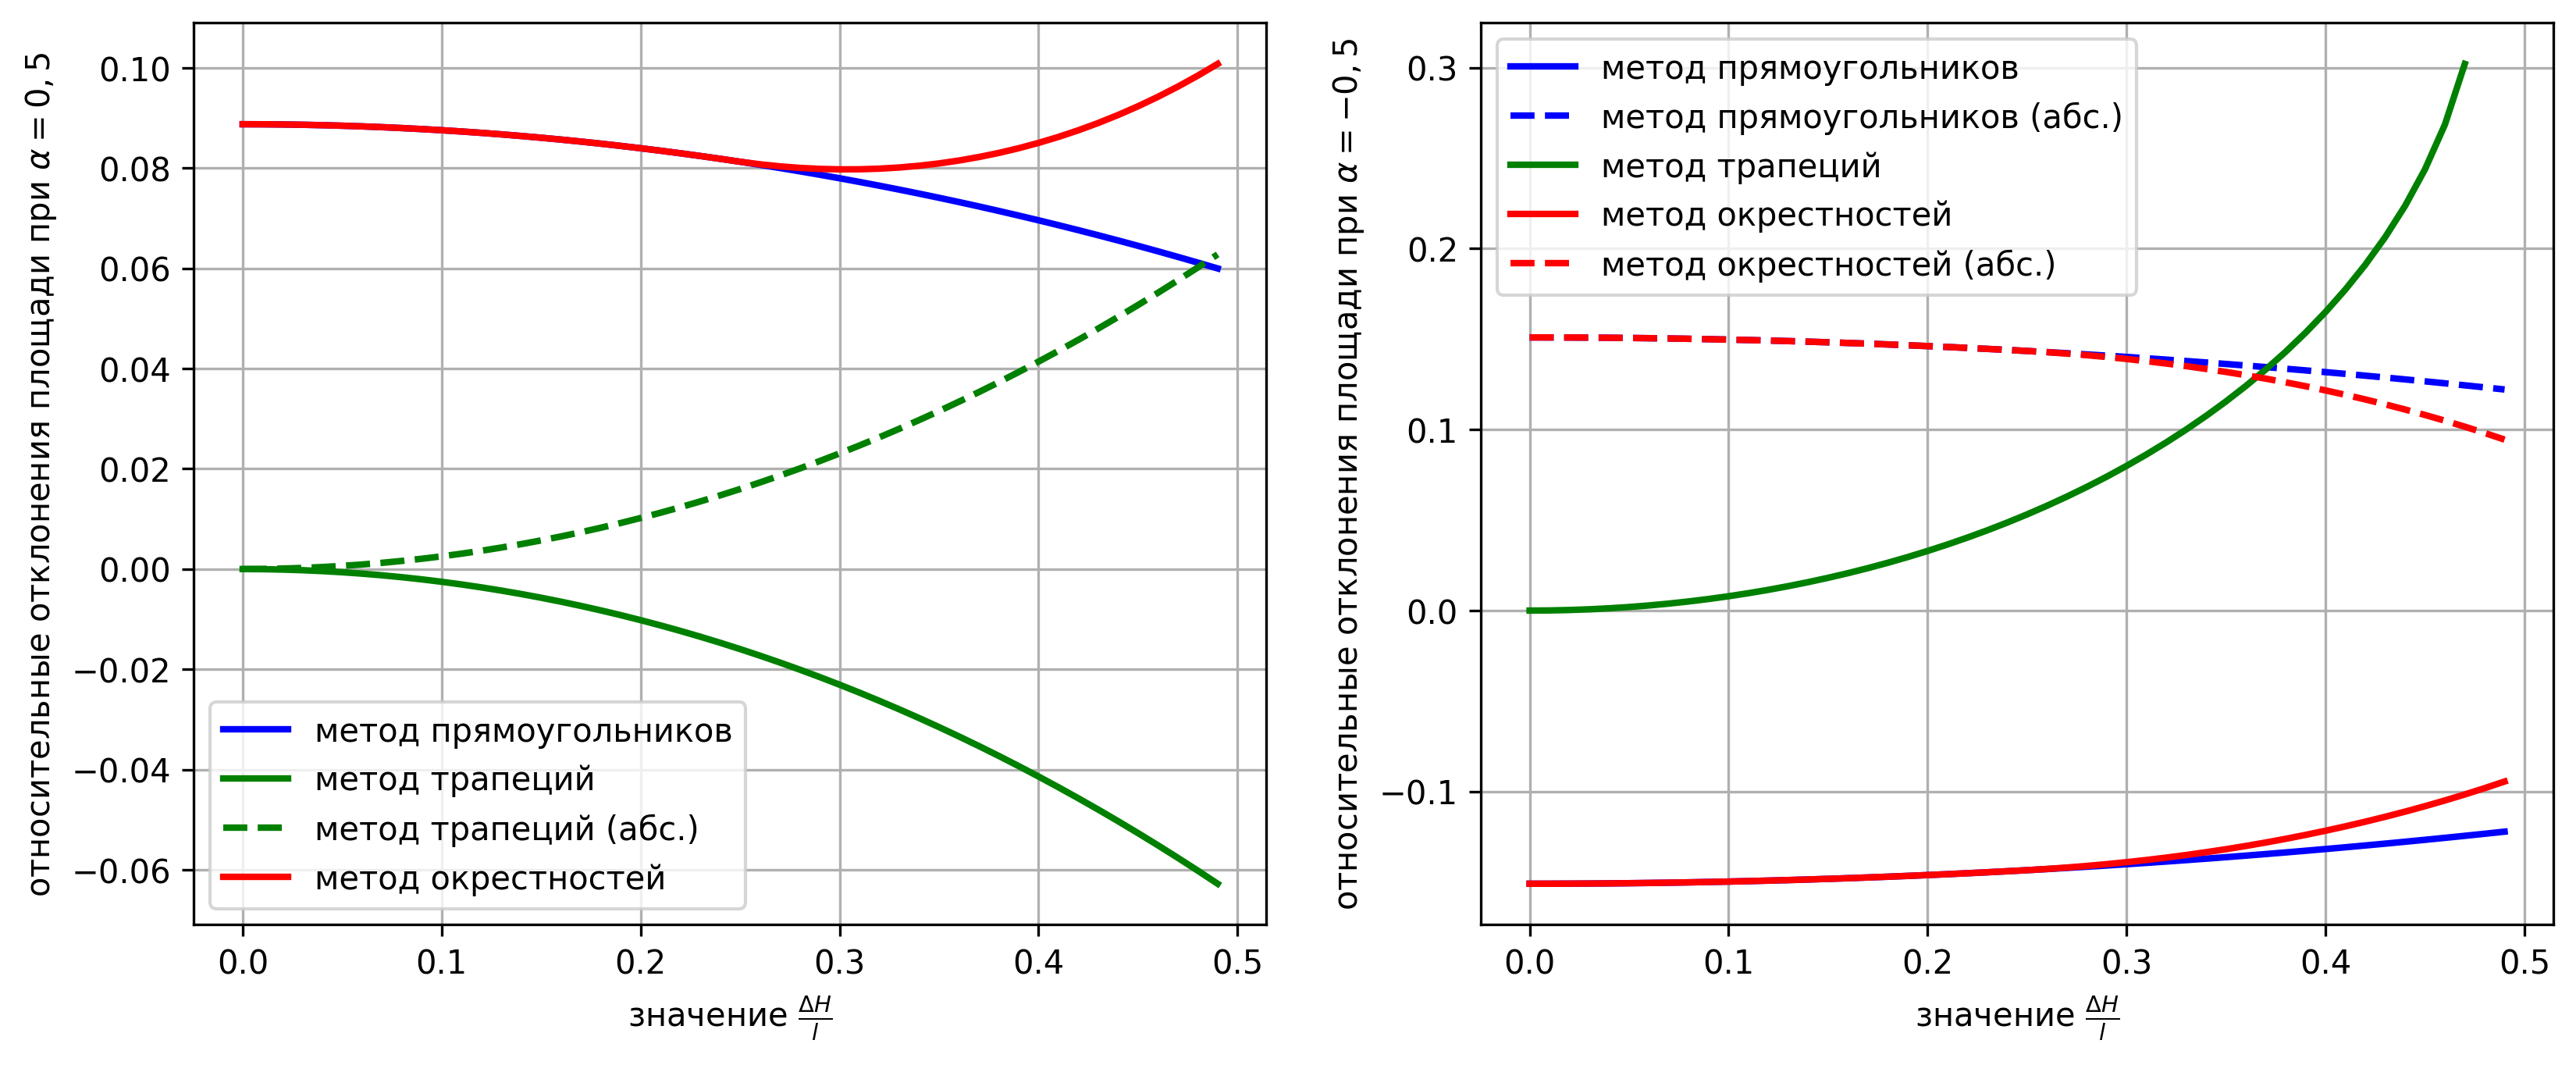
\includegraphics[width=1.0\textwidth]{pics/remesh_fix_alfa_chart.png}
\captionstyle{normal}\caption{Charts of $\delta_i^r(\frac{\Delta H}{l})$, $\delta_i^t(\frac{\Delta H}{l})$, $\delta_i^o(\frac{\Delta H}{l})$ for fixed values of $\alpha = 0.5$ (left) and $\alpha = -0.5$ (right).}
\label{fig:text_1_remesh_fix_alfa_chart}
\end{figure}

%--------------------------------------------------------------------------------------------------------------------------------

\section{Smoothing out sharp peaks and caverns}

Let us present estimates of smoothing of sharp peaks and caverns for the considered methods of mesh rebuilding (rectangles, trapeziums and neighborhoods methods). For this, we will consider a computational mesh with identical cells-segments of length $l$.

To evaluate the smoothing of sharp peaks, we will assume that the mesh is absolutely flat except for two adjacent cells that form a sharp peak with an angle of $2 \alpha$ (see Fig.~\ref{fig:text_1_remesh_2d_peak_cavern_general} on the left).
Similarly, to evaluate the smoothing of caverns, we will assume that the mesh is absolutely flat except for two adjacent cells that form a valley with an angle of $2 \alpha$ (see Fig.~\ref{fig:text_1_remesh_2d_peak_cavern_general} on the right).

\begin{figure}[ht]
\setcaptionmargin{5mm}
%\onelinecaptionsfalse % if the caption is multiline
\onelinecaptionstrue  % if the caption is one-line
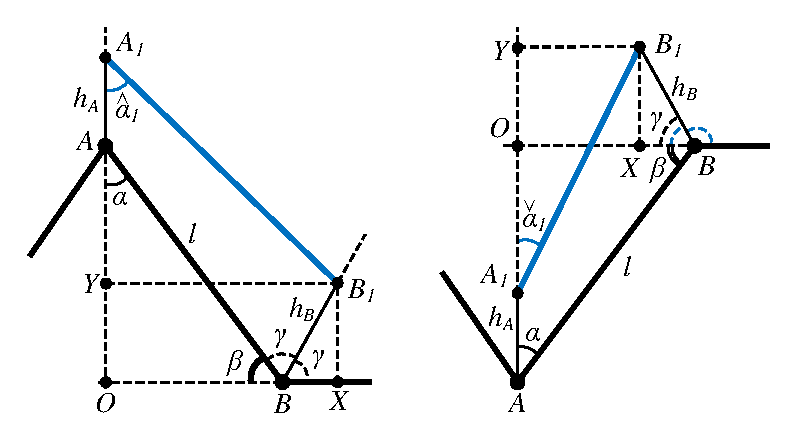
\includegraphics[width=0.8\textwidth]{./pics/peak-cavern-general.pdf}
\captionstyle{normal}\caption{Evaluation of angle smoothing at a sharp peak (left) and at a trough (right).}
\label{fig:text_1_remesh_2d_peak_cavern_general}
\end{figure}

In all three methods (rectangles, trapeziums and neighborhoods) the directions of node displacement coincide (and lie on the bisectors of the angles formed by neighboring cells), so we will consider the problem of smoothing the angle at a sharp peak and at a cavern for arbitrary displacements of nodes $A$ and $B$. To do this, we will prove the following lemmas.

\begin{lemma}\label{lem:text_1_peak_smooth}
When moving nodes $A$ and $B$ -- nodes of one of the sides of the sharp peak -- along the bisectors of the angles formed by the incident cells, by distances $h_A$ and $h_B$, respectively (see Fig.~\ref{fig:text_1_remesh_2d_peak_cavern_general} on the left), the value of the smoothed angle $\angle OA_1B_1 = \hat{\alpha}_1$ is expressed through $\angle OAB = \alpha$ as follows:
\begin{equation}\label{eqn:text_1_envelope_alpha1_peak}
\hat{\alpha}_1(h_A, h_B) = \arctg \frac{l \sin \alpha + h_B \cos \gamma}{l \cos \alpha + h_A - h_B \sin \gamma}	
\end{equation}
\end{lemma}

Let's express the remaining angles through $\alpha$: $\beta = \frac{\pi}{2} - \alpha$, $\gamma = \frac{\pi}{4} + \frac{\alpha}{2}$. Using the angles $\alpha$ and $\gamma$ we find $OA = l \cos \alpha$, $OB = l \sin \alpha$, $BX = h_B \cos \gamma$, $B_1X = h_B \sin \gamma = OY$, whence we obtain $YB_1 = OB + BX = l \sin \alpha + h_B \cos \gamma$, $YA_1 = OA + AA_1 - OY = l \cos \alpha + h_A - h_B \sin \gamma$, whence we obtain $\hat{\alpha}_1(h_A, h_B) = \arctg \frac{YB_1}{YA_1}$, which leads to \eqref{eqn:text_1_envelope_alpha1_peak}.
$\blacksquare$\\

\begin{lemma}\label{lem:text_1_cavern_smooth}
When moving nodes $A$ and $B$ -- nodes of one of the sides of the cavern -- along the bisectors of the angles formed by the incident cells, by distances $h_A \le AO$ and $h_B$, respectively (see Fig.~\ref{fig:text_1_remesh_2d_peak_cavern_general} on the right), the value of the smoothed angle $\angle OA_1B_1 = \check{\alpha}_1$ is expressed through $\angle OAB = \alpha$ as follows:
\begin{equation}\label{eqn:text_1_envelope_alpha1_cavern}
\check{\alpha}_1(h_A, h_B) = \arctg \frac{l \sin \alpha - h_B \cos \gamma}{l \cos \alpha - h_A + h_B \sin \gamma}
\end{equation}
under constraints on the angle $\alpha$
\begin{equation}\label{eqn:text_1_envelope_alpha1_cavern2}
\arcsin \frac{h_B \left( \sqrt{8 l^2 + h_B^2} - h_B \right)}{4 l^2} \le \alpha \le \arccos \frac{h_A}{l}
\end{equation}
\end{lemma}

Let's express the remaining angles through $\alpha$: $\beta = \frac{\pi}{2} - \alpha$, $\gamma = \frac{\pi}{4} + \frac{\alpha}{2}$. Using angles $\alpha$ and $\gamma$ we find $OA = l \cos \alpha$, $OB = l \sin \alpha$, $BX = h_B \cos \gamma$, $B_1X = h_B \sin \gamma = OY$, whence we obtain $YB_1 = OB - BX = l \sin \alpha - h_B \cos \gamma$, $YA_1 = OA - AA_1 + OY = l \cos \alpha - h_A + h_B \sin \gamma$, whence we obtain $\check{\alpha}_1(h_A, h_B) = \arctg \frac{YB_1}{YA_1}$, which leads to \eqref{eqn:text_1_envelope_alpha1_cavern}.

Let us consider additional conditions for the applicability of the formula \eqref{eqn:text_1_envelope_alpha1_cavern}.

The condition $h_A \le AO$ is equivalent to $\alpha \le \arccos \frac{h_A}{l}$.

The requirement for the absence of self-intersection of the mesh is the condition $BX \le OB$, that is, $h_B \cos \gamma \le l \sin \alpha$.
Substituting the explicit expression for $\cos \gamma$, we obtain
\begin{equation}
	h_B \frac{1}{\sqrt{2}} \left( \cos \frac{\alpha}{2} - \sin \frac{\alpha}{2} \right) \le l \sin \alpha
\end{equation}

Since $\alpha < \frac{\pi}{2}$, both parts of the inequality are positive, so we square them, and after transformations we get
\begin{equation}\label{eqn:text_1_envelope_find_alpha3}
	1 - \sin \alpha \le 2 \left( \frac{l}{h_B} \right)^2 \sin^2 \alpha
\end{equation}

Introducing the notation $p = 2 \left( \frac{l}{h_B} \right)^2$ and solving the quadratic inequality \eqref{eqn:text_1_envelope_find_alpha3} with respect to $\sin \alpha$, we obtain the condition $\alpha \ge \arcsin \frac{\sqrt{4p + 1} - 1}{2p}$, which together with the condition $\alpha \le \arccos \frac{h_A}{l}$ leads to \eqref{eqn:text_1_envelope_alpha1_cavern2}.
$\blacksquare$\\

\begin{figure}[ht]
\setcaptionmargin{5mm}
\onelinecaptionsfalse % if the caption is multiline
%\onelinecaptionstrue  % if the caption is one-line
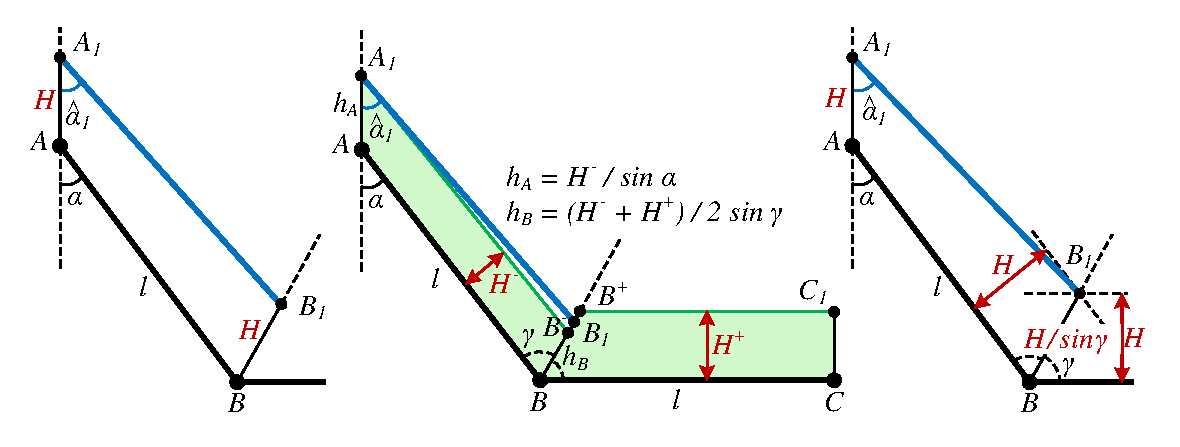
\includegraphics[width=1.0\textwidth]{./pics/peak-methods.pdf}
\captionstyle{normal}\caption{Smoothing of the peak using the rectangles (left), trapeziums (center), and neighborhoods (right) methods.}
\label{fig:text_1_remesh_2d_peak_methods}
\end{figure}

\begin{figure}[ht]
\setcaptionmargin{5mm}
%\onelinecaptionsfalse % if the caption is multiline
\onelinecaptionstrue  % if the caption is one-line
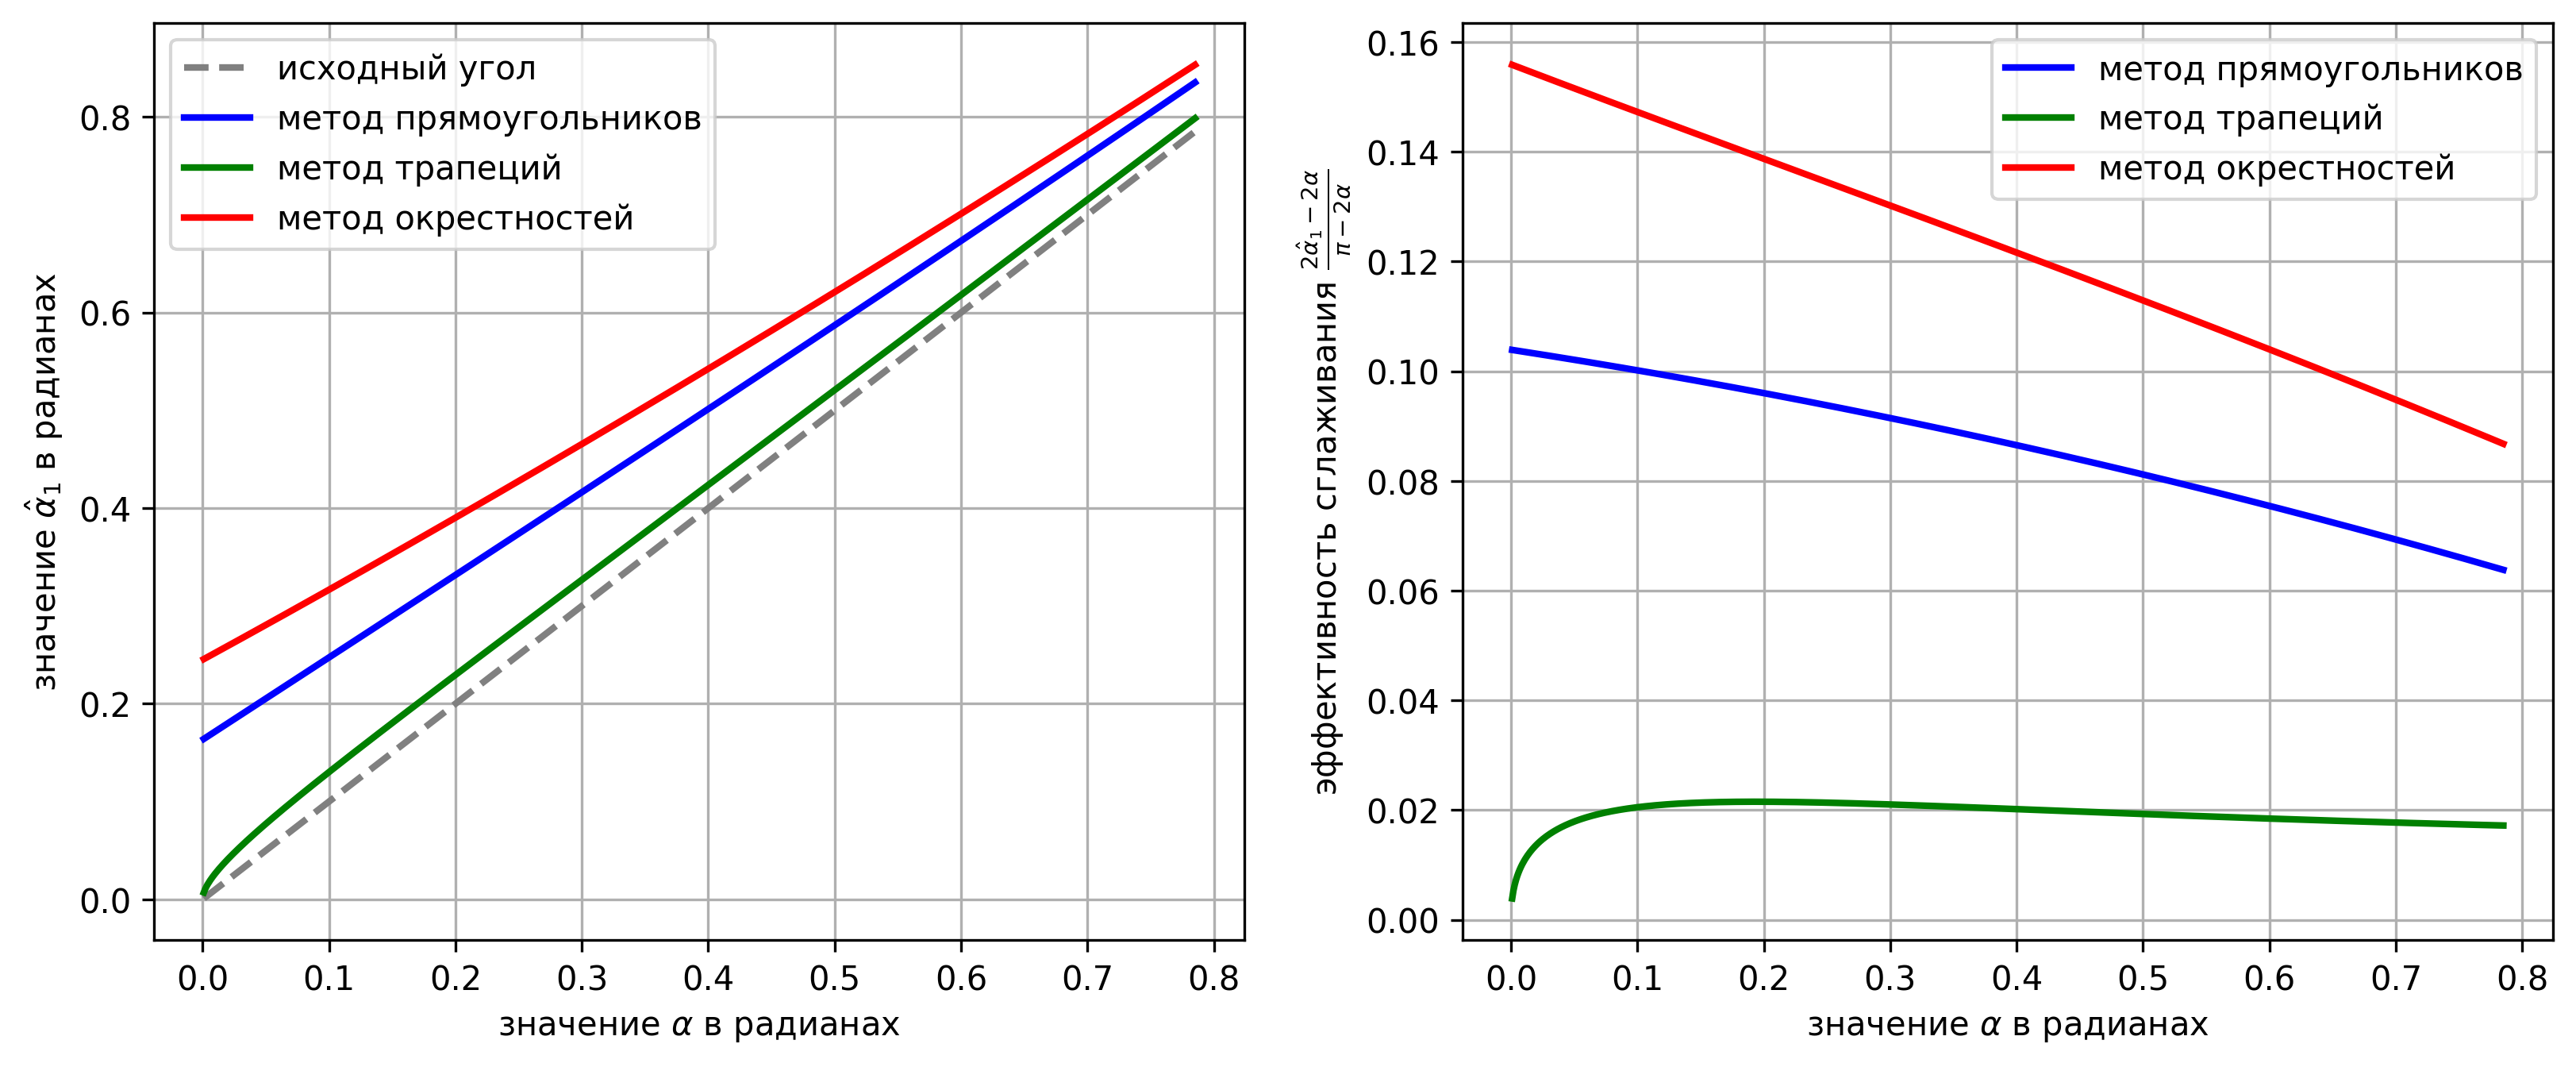
\includegraphics[width=1.0\textwidth]{./pics/peak-methods-chart.png}
\captionstyle{normal}\caption{Comparison of sharp peak smoothing for rectangles, trapeziums and neighborhoods methods.}
\label{fig:text_1_remesh_2d_peak_methods_chart}
\end{figure}

Based on Lemma~\ref{lem:text_1_peak_smooth}, we obtain estimates of the smoothing of the angle at a sharp peak under the condition of a constant value of $H$ in all mesh cells.

For the rectangles method we have $h_A = h_B = H$ (see Fig~\ref{fig:text_1_remesh_2d_peak_methods} on the left).

For the trapeziums method, it is necessary to first find the heights of the trapeziums $AA_1B^{-}B$ and $CC_1B^{+}B$ from Fig.~\ref{fig:text_1_remesh_2d_peak_methods} in the center from the condition that the areas of these trapeziums are equal to the value of $lH$.
The heights of these trapeziums $H^{-}$ and $H^{+}$ are obtained by solving a quadratic equation.
Then $h_A = \frac{H^{-}}{\sin \alpha}$, $h_B = \frac{H^{-} + H^{+}}{2 \sin \gamma}$.

In the case of the neighborhoods method $h_A = H$, $h_B = \frac{H}{\sin \gamma}$ (see Fig.~\ref{fig:text_1_remesh_2d_peak_methods} on the right).

Fig.~\ref{fig:text_1_remesh_2d_peak_methods_chart} shows comparison charts of rectangles, trapeziums and neighborhoods methods applied to smoothing sharp peaks.
In this case, a fixed cell offset value $H = \frac{l}{4}$ is used.
The chart on the left shows the dependence of the change in the smoothed angle $\hat{\alpha}_1$ on $\alpha$.
The chart on the right shows the smoothing efficiency expressed by the formula $\frac{2 \hat{\alpha}_1 - 2 \alpha}{\pi - 2 \alpha}$ (the value 1 means complete smoothing of the peak up to the angle $\hat{\alpha}_1 = \frac{\pi}{2}$).

It can be noted that the most effective smoothing of the angle $\alpha$ is provided by the neighborhoods method.
Additionally, we note that using the trapeziums method for small angles $\alpha$ leads to an uncontrolled growth of $h_A$, which makes the use of this method unacceptable.

\begin{figure}[ht]
\setcaptionmargin{5mm}
\onelinecaptionsfalse % if the caption is multiline
%\onelinecaptionstrue  % if the caption is one-line
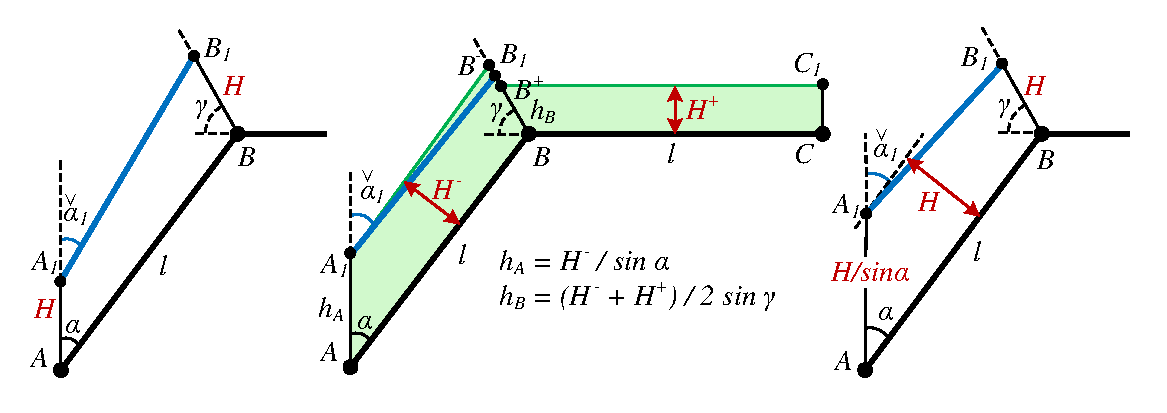
\includegraphics[width=1.0\textwidth]{./pics/cavern-methods.pdf}
\captionstyle{normal}\caption{Smoothing of a cavern using the rectangles (left), trapeziums (center), and neighborhoods (right) methods.}
\label{fig:text_1_remesh_2d_cavern_methods}
\end{figure}

\begin{figure}[ht]
\setcaptionmargin{5mm}
%\onelinecaptionsfalse % if the caption is multiline
\onelinecaptionstrue  % if the caption is one-line
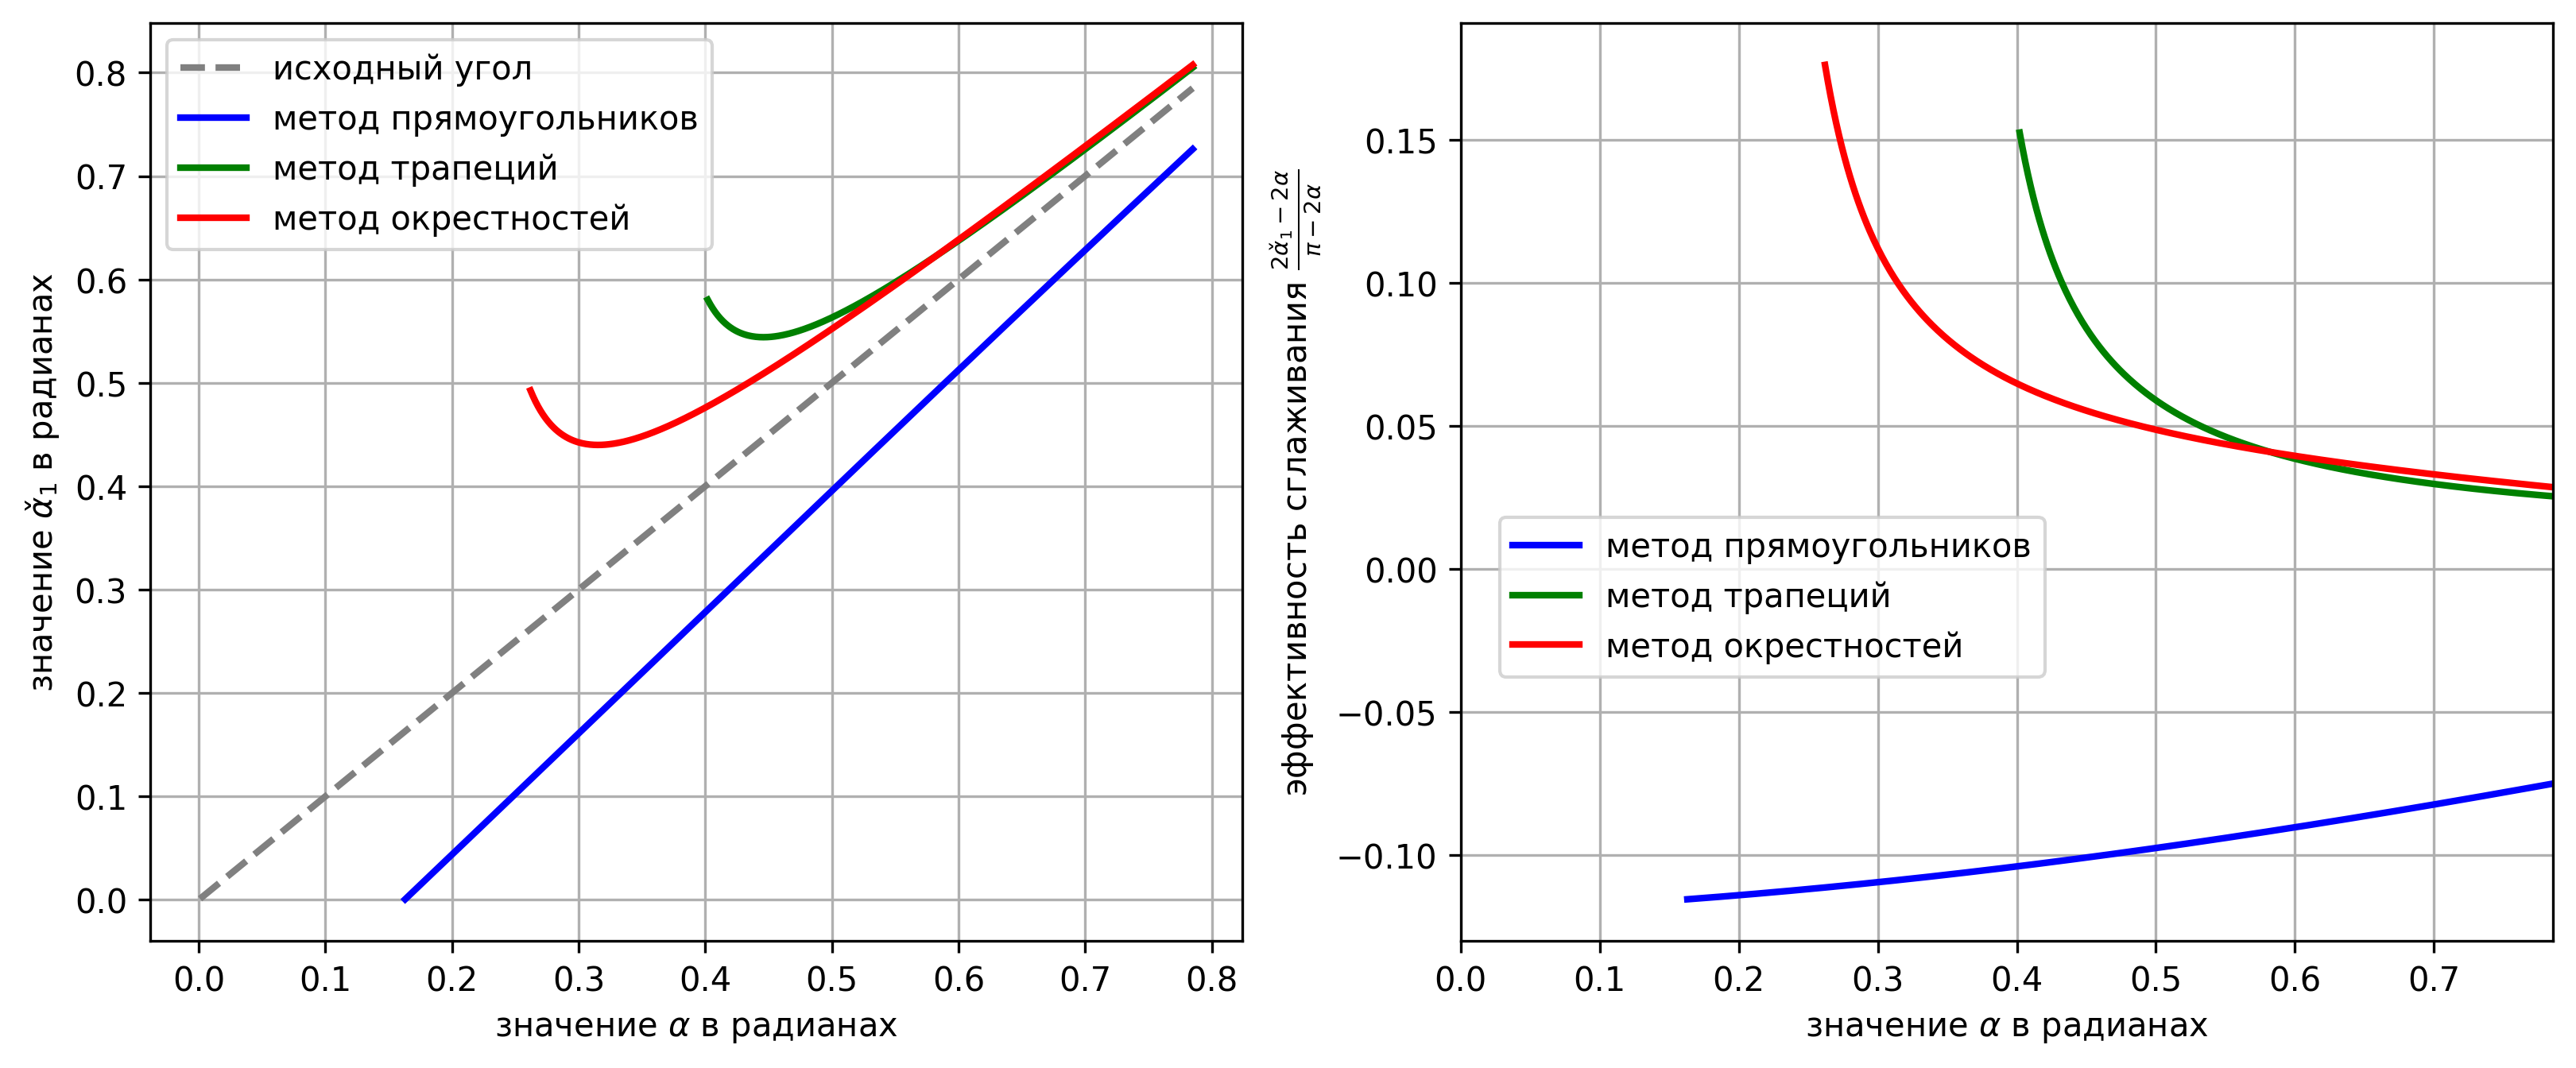
\includegraphics[width=1.0\textwidth]{./pics/cavern-methods-chart.png}
\captionstyle{normal}\caption{Comparison of cavern smoothing for rectangles, trapeziums and neighborhoods methods.}
\label{fig:text_1_remesh_2d_cavern_methods_chart}
\end{figure}

Based on Lemma~\ref{lem:text_1_cavern_smooth}, we obtain estimates of the smoothing of an angle at a cavern under the condition of a constant value of $H$ in all mesh cells.

For the rectangles method we have $h_A = h_B = H$ (see Fig~\ref{fig:text_1_remesh_2d_cavern_methods} on the left).

For the trapeziums method, it is necessary to first find the heights of the trapeziums $AA_1B^{-}B$ and $CC_1B^{+}B$ from Fig.~\ref{fig:text_1_remesh_2d_cavern_methods} in the center from the condition that the areas of these trapeziums are equal to the value of $lH$.
The heights of these trapeziums $H^{-}$ and $H^{+}$ are obtained by solving a quadratic equation.
Then $h_A = \frac{H^{-}}{\sin \alpha}$, $h_B = \frac{H^{-} + H^{+}}{2 \sin \gamma}$.

In the case of the neighborhoods method $h_A = \frac{H}{\sin \alpha}$, $h_B = H$ (see Fig.~\ref{fig:text_1_remesh_2d_cavern_methods} on the right).

Fig.~\ref{fig:text_1_remesh_2d_cavern_methods_chart} shows comparison charts of rectangles, trapeziums and neighborhoods methods applied to smoothing of caverns.
In this case, a fixed cell offset value $H = \frac{l}{4}$ is used.
The chart on the left shows the dependence of the change in the smoothed angle $\check{\alpha}_1$ on $\alpha$.
The chart on the right shows the smoothing efficiency expressed by the formula $\frac{2 \check{\alpha}_1 - 2 \alpha}{\pi - 2 \alpha}$ (the value 1 means complete smoothing of the peak up to the angle $\hat{\alpha}_1 = \frac{\pi}{2}$).

It can be noted that the rectangles method does not smooth the angle, but on the contrary, makes it even sharper (the smoothing efficiency value is less than zero).
The trapeziums method shows better smoothing efficiency, but with a smaller area of ​​applicability.

%--------------------------------------------------------------------------------------------------------------------------------

\section{Conclusion}

The following conclusions can be drawn from the above estimates of the accuracy of the surface mesh rebuilding methods (see Fig.~\ref{fig:text_1_remesh_3d_main_chart}), as well as the ability to smooth out sharp peaks (see Fig.~\ref{fig:text_1_remesh_2d_peak_methods_chart}) and caverns (see Fig.~\ref{fig:text_1_remesh_2d_cavern_methods_chart}).
The trapeziums mesh rebuilding method is more accurate, the accuracy of the rectangles and neighborhoods methods is almost the same for small values ​​and changes in $H$.
From the point of view of smoothing out mesh defects, the trapeziums method is not applicable, since it leads to uncontrolled growth of sharp peaks.
The rectangles method is ineffective in smoothing out sharp peaks and is not capable of smoothing out caverns.
Thus, the neighborhoods rebuilding method is optimal in terms of rebuilding accuracy and the ability to smooth out mesh defects.

%--------------------------------------------------------------------------------------------------------------------------------

\begin{acknowledgments}
The work was carried out as part of the state assignment of the National Research Centre \textquotedblleft Kurchatov Institute\textquotedblright.

\end{acknowledgments}

%
% The Bibliography
%

\begin{thebibliography}{99}

\bibitem{Raj}
\refitem{article}
L.~Prince~Raj, K.~Yee, and R.~S.~Myong, \textquotedblleft Sensivity of ice and aerodynamic performance degradation to critical physical and modeling parameters affecting airfoil icing\textquotedblright, Aerospace Sci. Technol. \textbf{98}, 105659-1--46 (2020). https://doi.org/10.1016/j.ast.2019.105659

\bibitem{Martini}
\refitem{article}
F.~Martini, H.~Ibrahim, L.~T.~C. Montoya, P.~Rizk, and A.~Ilinca, \textquotedblleft Turbulence modeling of iced wind turbine airfoils\textquotedblright, Energies \textbf{15}, 8325-1--21 (2022). https://doi.org/10.3390/en15228325

\bibitem{Koshelev}
\refitem{article}
K.~B.~Koshelev, V.~G.~Melnikova, and S.~V.~Strijhak, \textquotedblleft Development of ice-foam solver for modeling ice accretion\textquotedblright, Tr. Inst. Sist. Program. RAN \textbf{32}, 217--234 (2020). https://doi.org/10.15514/ISPRAS-2020-32(4)-16

\bibitem{Sorokin}
\refitem{article}
K.~E.~Sorokin, P.~M.~Byvaltsev, A.~A.~Aksenov, S.~V.~Zhluktov, D.~V.~Savitskiy, A.~A.~Babulin, and V.~I.~Shevyakov, \textquotedblleft Numerical simulation of ice accretion if FlowVision sotfware\textquotedblright, Comput. Res. Model. \textbf{12}, 83--96 (2020). https://doi.org/10.20537/2076-7633-2020-12-1-83-96

\bibitem{Galanov}
\refitem{article}
N.~G.~Galanov, A.~V.~Sarazov, R.~N.~Zhukov, and A.~S.~Kozelkov, \textquotedblleft Application of various ice accretion simulation approaches in the LOGOS software package\textquotedblright, J. Phys.: Conf. Ser. \textbf{2099}, 012029-1--8 (2021). https://doi.org/10.1088/1742-6596/2099/1/012029

\bibitem{Bartkus}
\refitem{article}
T.~P.~Bartkus, P.~M.~Struk, and J.-C.~Tsao, “Evaluation of a thermodynamic ice-crystal icing model using experimental ice accretion data,” in \textit{Proceedings of the Atmospheric and Space Environments Conference, 2018, pp. 1--18}. https://doi.org/10.2514/6.2018-4129

\bibitem{Zhang}
\refitem{article}
X.~Zhang, X.~Wu, and J.~Min, “Aircraft icing model considering both rime ice property variability and runback water effect,” Int. J. Heat Mass Transfer \textbf{104}, 510--516 (2017). https://doi.org/10.1016/j.ijheatmasstransfer.2016.08.086

\bibitem{Pena}
\refitem{article}
D.~Pena, Y.~Hoarau, and E.~Laurendeau, “A single step ice accretion model using level-set method,” J. Fluids Struct. \textbf{65}, 278--294 (2016). https://doi.org/10.1016/j.jfluidstructs.2016.06.001

\bibitem{Beaugendre}
\refitem{misc}
H.~Beaugendre, \textquotedblleft A PDE-based approach to in-flight ice accretion\textquotedblright, PhD Thesis (Dep. of Mech. Eng., McGill Univ., Montr\'eal, Qu\'ebec, 2003).

\bibitem{Tong}
\refitem{article}
X.~Tong, D.~Thompson, Q.~Arnoldus, E.~Collins, and E.~Luke, \textquotedblleft Three-dimensional  surface evolution and mesh deformation for aircraft icing applications\textquotedblright, J. of Aircraft {\bf 54}, 1047--1063 (2017). https://doi.org/10.2514/1.C033949

\bibitem{Rybakov}
\refitem{article}
A.~A.~Rybakov and S.~S.~Shumilin, \textquotedblleft Approximate  methods of the surface mesh deformation in two-dimensional case\textquotedblright, Lobachevskii J. Math. {\bf 40}, 1848--1852 (2019). https://doi.org/10.1134/S1995080219110258

\bibitem{Meshcheryakov}
\refitem{article}
A.~O.~Meshcheryakov, and A.~A.~Rybakov, \textquotedblleft Evolution of the surface computational mesh in the ice accretion process\textquotedblright, Lobachevskii J. Math. {\bf 44}, 361--378 (2023). https://doi.org/10.1134/S1995080223110367

\end{thebibliography}
\end{document}
